\documentclass[11pt,a4paper]{article}
\usepackage{fontspec}
% xeCJK intentionally omitted for now: this paper carries no CJK glyphs yet.
% Re-add \usepackage{xeCJK}\setCJKmainfont{...} (with a font tectonic can find)
% when a token example such as the raw-mode crystal is shown inline.
\usepackage{amsmath,amssymb,amsthm}
\usepackage{graphicx}
\usepackage{booktabs}
\usepackage{hyperref}
\usepackage{xcolor}
\usepackage{geometry}
\usepackage{enumitem}
\usepackage{multirow}
\usepackage{float}
\usepackage{longtable}
\geometry{margin=1in}

% --- The provenance apparatus: this paper's signature. Every figure states the
% .mri it was measured from and the script that captured it, so figure and datum
% are one object, regenerable on demand. This is the whole point of an agent
% that can drive the instrument AND photograph it in the same session. ---
\definecolor{prov}{RGB}{95,95,95}
\newcommand{\provenance}[1]{\par\vspace{2pt}{\footnotesize\ttfamily\textcolor{prov}{#1}}}
\newcommand{\heinrich}{\textsc{Heinrich}}
\newcommand{\mri}{\texttt{.mri}}

\title{The Frozen Frame\\[0.5em]\large An Instrument That Measures a Language Model\\Against a Ruler Made From Itself}

\author{Built by Claude instances, steered by a human, measured by machines\\
Toolkit: \heinrich{}\\[0.5em]
\small The first Heinrich paper whose figures were captured, not drawn---\\
each rendered from the same run, in the same frame, that produced its numbers.}

\date{July 2026 --- draft}

\begin{document}
\maketitle

\begin{abstract}
The previous Heinrich papers were about what models do. This one is about how to
know. They shared a hidden dependency: every geometric claim was measured against
a coordinate system that the measurement could itself move. A safety direction, a
displacement, a trajectory---each was read off a frame re-derived from the data at
hand, so the ruler flexed with the thing it measured. This paper describes the
instrument built to stop that. A per-layer PCA frame is computed once over the
model's own vocabulary and never re-derived; the number of retained components
equals the hidden width and the components are orthonormal, so distance in the
score coordinates \emph{is} distance in the hidden state, exactly. Every token---any
of the tens of thousands---then holds a fixed address, and any live forward pass can
be measured against all of them at once with no truncation anywhere in the metric.
The instrument declares where it cannot be trusted: a per-layer noise floor from
\texttt{float16} forward reproducibility, and a frame-validity test by principal
angles against a held-out projection. And it renders every measurement as a
navigable surface an agent can drive and photograph, so a figure in this paper and
the number beside it come from one session and one frame. We demonstrate the
instrument on a single question---during a forward pass, does the residual migrate
toward the token it will emit?---and answer it: no. The state does not travel to the
answer; it rotates to aim at it. We close with what the instrument cannot do, and
why that ceiling is a property of the method, not of the hardware.
\end{abstract}

\tableofcontents
\newpage

%==============================================================
\section{What This Document Is}
%==============================================================

The prior papers in this series measured behaviour: which models refuse, which
break, how safety is arranged in the residual stream. \heinrich{} v3 ended on a
confession---every measurement error it had made pushed in the same direction,
making models look safer than they were, because the investigator shared training
lineage with the investigated. The lesson was not ``we found the right number this
time.'' The lesson was that a measurement instrument must be able to state its own
bias, or it will quietly encode the measurer's.

This document is the instrument built from that lesson. It is not about safety, or
any one model, or any one finding. It is about a ruler: how to hold a language
model's internal geometry still enough to measure, how to prove the ruler has not
moved, and how to publish a measurement so that its picture and its number cannot
drift apart. The finding we use to exercise it---that a model \emph{aims} at its
next token rather than \emph{travelling} to it---is a worked example, chosen because
it is the cleanest thing the ruler has shown us, not because the paper is about it.

A note on the figures. This is the first Heinrich paper with any. Every earlier one
was prose and tables because a hand-made figure is a claim you cannot check: the
picture is drawn to illustrate a number computed elsewhere, and nothing binds them.
Here an agent runs the measurement and then drives the live instrument to photograph
the exact state that measurement produced. The picture and the number are the same
event. Each figure carries, in monospace beneath its caption, the \mri{} it came
from and the script that captured it. None of them are drawn.

%==============================================================
\section{The Problem: A Ruler That Moves}
%==============================================================

To compare two hidden states---this layer to that layer, this token to the answer
token---you need a coordinate system they share. The usual move is to fit one from
the data: PCA the activations you have, read the coordinates off the top components.
The trouble is that the frame then depends on \emph{which} activations you fed it. Add
prompts, change the sample, re-run the probe, and the axes rotate; a ``direction''
that was there at $n{=}8$ is gone at $n{=}15$ (v3 lost its safety layers exactly this
way). The ruler is a function of the thing being measured, so every distance is
contaminated by the choice of measuring set. Worse for trajectories: to ask whether a
live state is \emph{near} a particular token, that token must have coordinates in the
same frame---but a token you did not sample has no address at all.

What is required is a frame that (i) is fixed independently of any particular query,
(ii) gives every token an address, and (iii) preserves true distances, so that
``close in the picture'' means ``close in the model.'' The next section is that frame.

The field's standard readout confronts a cousin of this problem from the other
side. The logit lens reads a hidden state through the final unembedding and
returns gibberish at intermediate layers, because each layer ``speaks its own
language''; the tuned lens (Belrose et al., 2023) repairs this with a
\emph{learned} affine translator fit per layer. That is a second moving part---a
trained transform between the state and its reading. The frozen frame takes the
opposite route: an exact, trainless change of basis (below) that leaves every
distance untouched, so there is nothing to fit and nothing to fit \emph{to}.

%==============================================================
\section{The Frozen Frame}
%==============================================================

Capture the model's residual state once, at every layer, over a broad token sample,
and decompose each layer with PCA---but retain \emph{all} $D$ components, where $D$ is
the hidden width, and store the components $C_\ell$, the mean $\mu_\ell$, and the
silence baseline $b_\ell$. This frame is written to disk and never recomputed. A live
hidden state $h_\ell$ receives coordinates by the same fixed transform,
%
\[
s \;=\; (h_\ell - b_\ell - \mu_\ell)\,C_\ell^{\!\top},
\qquad C_\ell C_\ell^{\!\top} = I,
\qquad \lVert s - s' \rVert_2 \;=\; \lVert h_\ell - h'_\ell \rVert_2 .
\]
%
Because $C_\ell$ is a full-rank orthonormal basis, the projection is a lossless
rotation: the score-space $L_2$ distance is the hidden-space $L_2$ distance, with no
truncation approximation anywhere. The frame is not a summary of the state; it is a
change of basis for it.

The vocabulary is projected through this same frozen frame---every token, not a
sample---so each token id acquires a fixed per-layer address (\texttt{vocab\_scores}).
A live trajectory can therefore be compared, exactly, against the entire vocabulary at
every depth in one pass. The frame is the coordinate contract; the \mri{} file is the
artifact that carries it between the producer that captured it and any consumer that
reads it.

Two subtractions are load-bearing and easy to forget. The stored mean $\mu_\ell$
recentres the frame; the silence baseline $b_\ell$ removes the model's resting state.
Omitting either leaves a constant offset that, at some layers, dwarfs the signal by
more than an order of magnitude. Both are applied on every projection.

%==============================================================
\section{The Instrument Declares Its Limits}
%==============================================================

A distance is only meaningful above the noise of the machine that produced it.
\heinrich{} measures that noise directly: it re-captures the sample forward pass in
\texttt{float16} and compares to the stored scores, giving a per-layer reproducibility
floor. Distances at or below the floor are the arithmetic of the hardware, not the
model, and are drawn as such.

The frame's own validity is testable, not assumed. A second projection is derived from
a held-out, crystal-suppressed vocabulary sample, and its principal angles against the
frame are measured layer by layer; the variance-weighted overlap is reported as a
falsification statistic. On SmolLM2-135M (raw) the frame holds at $0.90$--$0.999$ at
every layer---stated as a licence to trust the ruler, revocable the moment a model
fails it.

% FIGURE (planned): frame-validity overlap curve + f16 noise-floor band, per layer.
% Data: web/.data/*/decomp/vocab_meta.json (frame_falsification, sample_agreement).
% Ready to capture now.

\subsection{Falsified against ground truth}

Self-declared trust is cheap unless the instrument can be caught fabricating. On
real language models there is no answer key. On a model we \emph{built} there is.
We tested the frame against matched causal-bank specimens---11.4M-parameter
models, deterministic substrate, pairs differing by exactly one flag
(normalisation on/off) at two seeds---built as a null case by the training-side
agent. Two tests, both adversarial by construction.

\emph{Artifact rate.} A re-capture of the same checkpoint is bit-identical (CKA
$1.000$): the instrument adds no noise of its own. So on a pair that differs by
exactly one flag, the entire reported gap is attributable to that flag---nothing
beyond the controlled variable is reported. It also orders causes correctly, which
a smearing frame would not: the flag effect (CKA $\approx0.59$) exceeds the
seed-only effect (CKA $\approx0.76$), which exceeds noise ($0$); by displacement
correlation the separation is starker still (seed $0.98$--$0.996$, flag
$0.69$--$0.71$).

\begin{table}[H]
\centering
\small
\begin{tabular}{llcc}
\toprule
comparison & varies & CKA & disp.\ corr \\
\midrule
re-capture of same checkpoint & nothing (noise floor) & \textbf{1.000} & \textbf{1.000} \\
same config, different seed    & seed only  & 0.73--0.79 & 0.98--0.996 \\
same seed, opposite flag       & flag only  & 0.58--0.60 & 0.69--0.71 \\
\bottomrule
\end{tabular}
\caption{The instrument against a ground-truth null. Zero noise floor, and the one
controlled variable (the flag) is the dominant reported difference---no structure
appears that is not traceable to a known cause.}
\label{tab:validation}
\end{table}

\emph{Does the method paint the cliff onto everything?} One tempting check is
worthless and we flag it as such: running the depth analysis on a depthless causal
bank returns an empty list, but only because the tool finds no per-layer files and
stops, having examined no data---it would return empty for any input of the wrong
shape. The real control runs the readout-cliff of Section~\ref{sec:worked} on a
transformer, against targets with no reason to commit. For ``The capital of France
is,'' the true answer commits at $0.77$ depth; of nine implausible words
(`` bicycle,'' `` velvet,'' `` thermostat,'' \ldots) not one commits at any layer
---each sits near the bottom of the sixteen-word panel from first layer to last.
Type-appropriate but wrong tokens (other capital cities) do eventually out-read the
random panel, but only at the final layer, never in the band. The three-quarters
commit is specific to the answer that fits; the method does not impose it on
arbitrary tokens---which is the property an empty list could never have shown.

%==============================================================
\section{The Shared Surface}
%==============================================================

The frame is not only a metric; it is a place. \heinrich{}'s companion renders the
frozen frame and any live trajectory as a navigable three-dimensional surface, and it
obeys one rule that makes its pictures admissible as evidence: \emph{omit, never fake}.
A segment renders only when both endpoints are genuinely in range; a candidate absent
from a layer's readout is not interpolated across the gap; every view states its own
sampling (``2{,}000 of 48{,}660'') and its own frame (``rel to live, $s{=}0.52$''). The
honesty is in the pixels, so a photograph of the surface carries its caveats into the
PDF.

This is what lets an agent produce figures that are measurements. The agent drives the
same instrument that computed the numbers, frames a view, and captures it in the same
session and the same frame. Figure~\ref{fig:horn} was made exactly this way.

%==============================================================
\section{Worked Example: Aiming, Not Traveling}
\label{sec:worked}
%==============================================================

We ask the instrument one question. During a forward pass, does the final-token
residual move toward the location of the token it is about to emit? The frozen frame
makes this answerable exactly: the answer token has a fixed address at every layer,
and so does the live state.

The proximity form of the hypothesis is false. Conditioned on the model actually
producing the answer, the answer token's own frozen state sits at roughly chance rank
among a background panel \emph{even at the final layer}: the trajectory does not go
there. The readout form is true. Reading each layer's state through the model's output
matrix, the answer out-competes the whole panel from a late band onward and at the
final layer without exception. The state does not approach the answer's location; it
rotates until it projects onto the answer's output direction. Distance-to-state and
preference-to-emit are different geometries---and the frozen frame is what let us hold
them apart. Figure~\ref{fig:horn} is that distinction made visible: a straight spine
that never bends toward a token, and a fan of readout candidates collapsing to the
commit.

\begin{figure}[H]
\centering
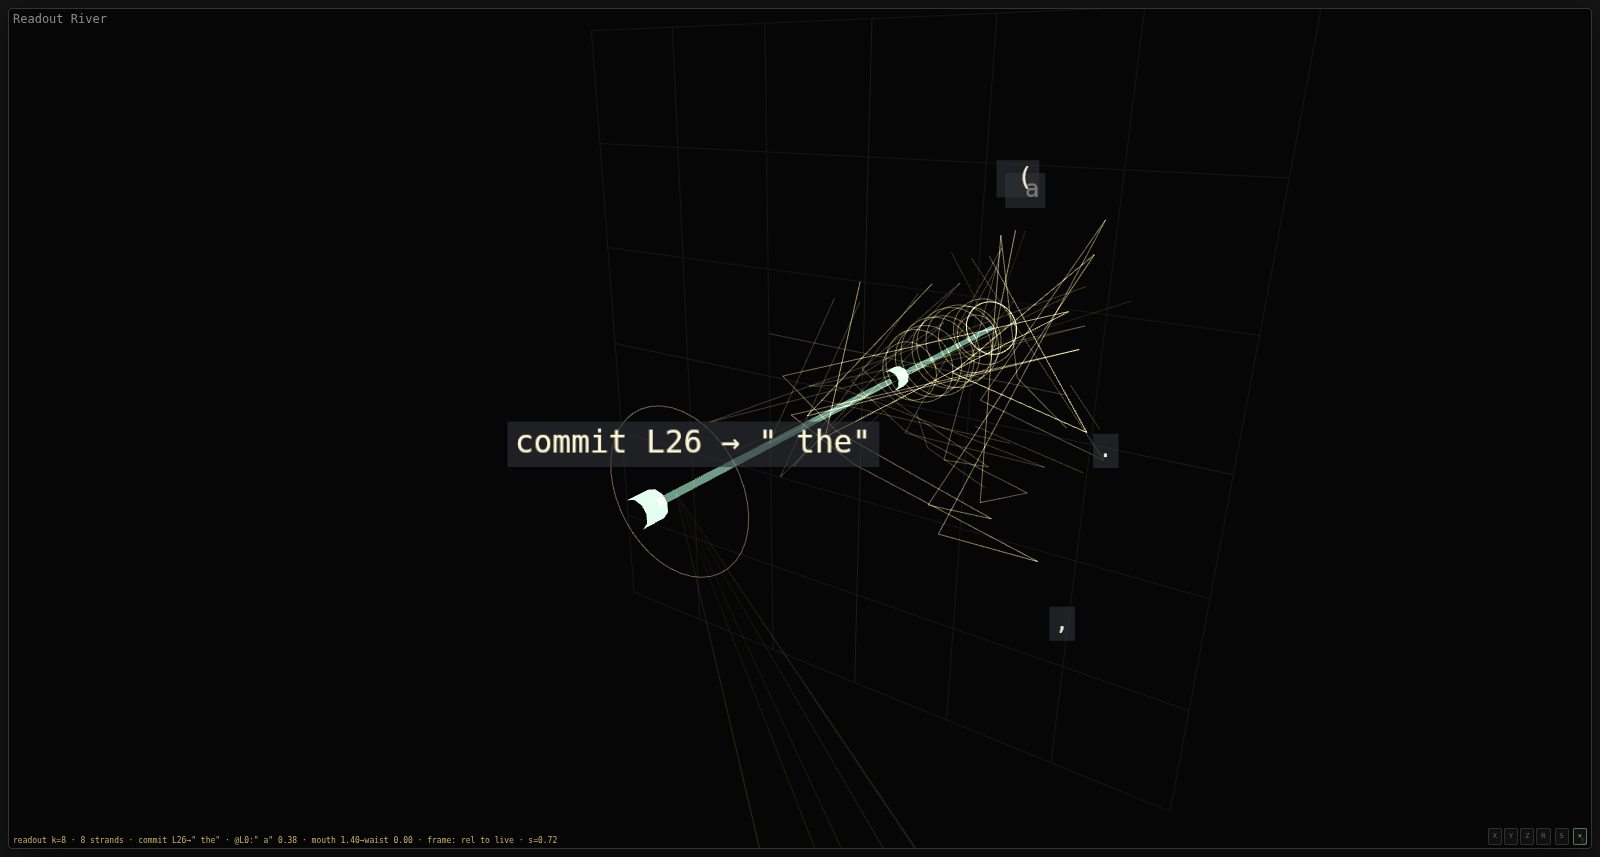
\includegraphics[width=0.94\textwidth]{figures/horn_smollm2-135m.png}
\caption{\textbf{The readout fan (``the horn'').} SmolLM2-135M (base), prompt
\textit{``The capital of France is,''} rendered in the frozen frame. The straight
teal spine is the live trajectory through depth; it runs down the axis and does not
bend toward any token's location. The gold fibers are the per-layer top-$k$ readout
candidates, each drawn at its true offset from the live state; they fan wide at the
mouth (early layers) and collapse to the commit at the waist (\texttt{L26}
$\rightarrow$ ``\,the''). A candidate absent from the top-$k$ between two layers is
not bridged---the fiber breaks rather than fake continuity. Labels resolve through the
full tokenizer (whitespace shown as a visible glyph, never a raw id).}
\label{fig:horn}
\provenance{mri: web/.data/smollm2-135m/raw.mri \quad{} capture: paper/figures/capture\_horn.mjs \quad{} readout: lmhead @ h/\textbar h\textbar}
\end{figure}

One horn is an anecdote. Replaying the identical protocol---twenty-eight
completion prompts, a sixteen-token background panel---on three further models,
one of them from a different tokenizer and architecture family, turns it into a
measurement. The answer out-reads the whole panel at the final layer in
twenty-seven to twenty-eight of twenty-eight runs on every model, so the readout
commit is not a one-model artifact. And the commit is scheduled by \emph{relative
depth}: the answer's rank collapses to zero near three-quarters of the way through
the network regardless of layer count---the median commit sits at 0.71--0.75 of
depth across models of 24, 30, and 32 layers---and regardless of family; Qwen, a
different tokenizer and architecture entirely, commits at the same fraction. Scale
buys correctness (the 360M model answers 24 of 28 versus 17 for the base 135M) but
not an earlier decision, and instruction tuning barely moves the band. The
instrument turned a single picture into a depth-invariant regularity that survives
a family boundary (Figure~\ref{fig:band}).

\begin{figure}[H]
\centering
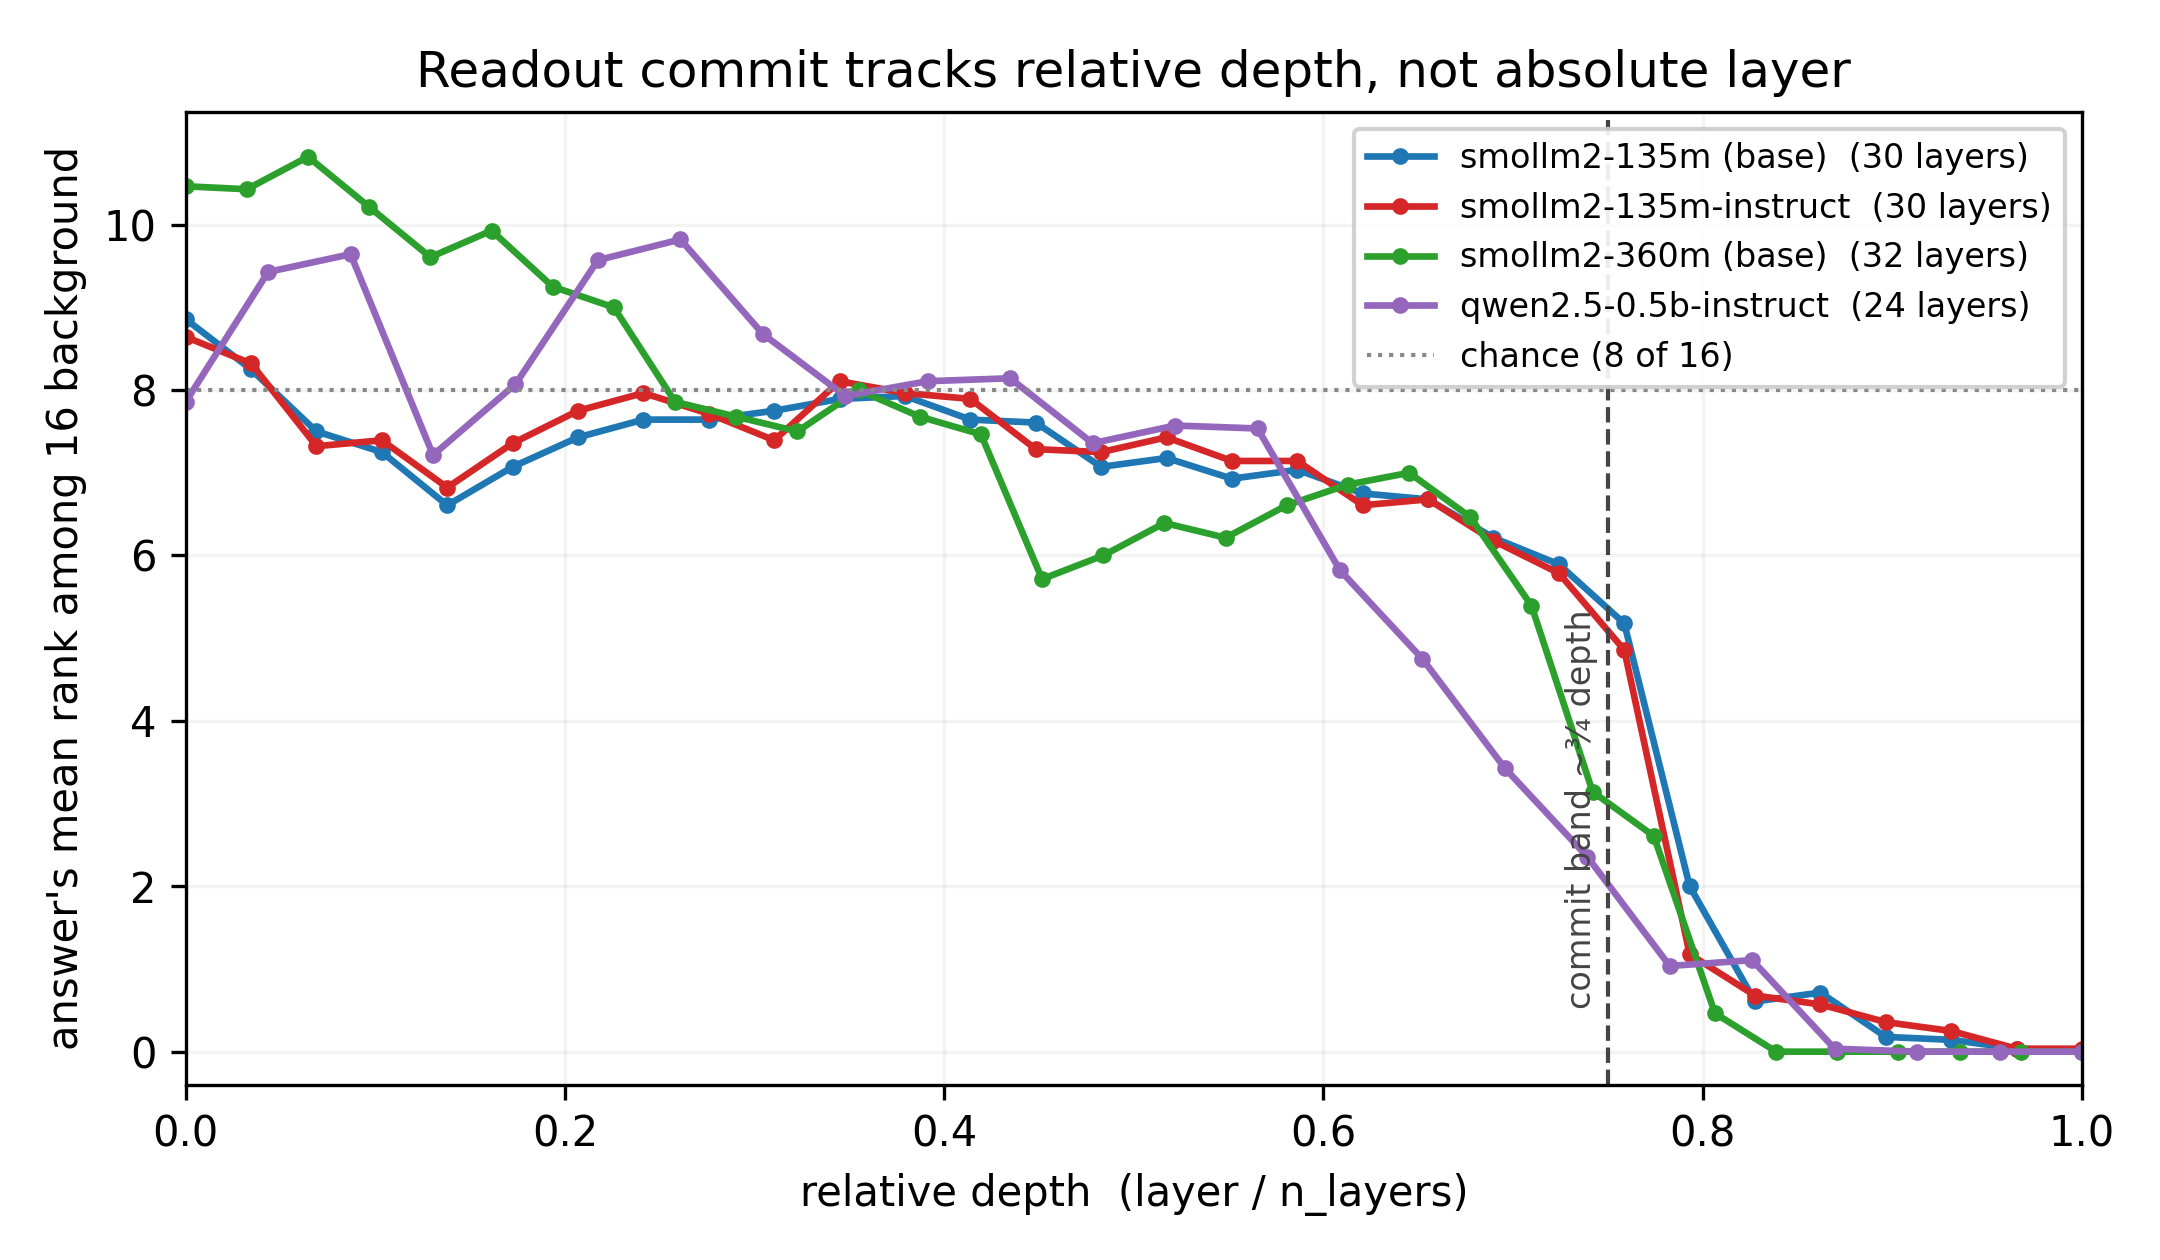
\includegraphics[width=0.92\textwidth]{figures/homing_band.png}
\caption{\textbf{The readout commit tracks relative depth.} For each model, the
answer token's mean rank among the sixteen-token background panel ($0$ = it
out-reads all of them) against relative depth (layer $/$ n\_layers). All three sit
near chance (8 of 16) through the first two-thirds of the network, then collapse
to rank $0$ in a narrow band at about three-quarters depth---across 24, 30, and 32
layers and two tokenizer families (SmolLM2 and Qwen), aligned only once depth is
normalised. The decision is scheduled by depth fraction, not absolute layer.}
\label{fig:band}
\provenance{data: docs/data/homing-study-v\{3,4\}*.json \quad{} run: scripts/homing\_study\_v4.py \quad{} plot: scripts/figure2\_homing\_band.py}
\end{figure}

This sits inside known structure, and the instrument's role is to sharpen a
distinction the standard tools blur. That prediction quality accrues smoothly, at
a fixed multiplicative rate per layer, regardless of architecture or scale, is an
established law of next-token prediction (arXiv:2408.13442, 2024). Our observation
is not that schedule but its complement: a specific answer's \emph{win} over its
competitors is not smooth at all but a late phase transition near three-quarters
depth, invisible to the aggregate residual that law measures. That the decision is
fixed internally well before the output echoes ``decide early, explain later''
(arXiv:2604.22266, 2026); that the state \emph{selects} rather than approaches its
token is the same position-versus-readout question a concurrent geometric account
is now asking (Lombardo et al., 2026), answered here with an exact hidden-space
distance rather than a lens. The instrument's claim is not a new law; it is that
these distinctions become measurable, and falsifiable, once the ruler holds still.

%==============================================================
\section{What the Instrument Cannot Do}
%==============================================================

The ceiling is not a matter of buying a bigger card. Faithful capture requires the
residual stream at full precision at every layer; the whole methodological claim is
that score distance is hidden distance \emph{exactly}. Quantising the weights or
offloading layers to fit a larger model trades that exactness away---the metric stops
being lossless the moment the numbers it reads are approximate. So the honest working
band is the range where full-precision internals are affordable (models up to a few
billion parameters on a single 12\,GB card), and the claims above are verified there
and stated as unverified above it. This is a scope, not a defeat: the structural
claims should hold at any scale for the same architectural reason, and the frozen
frame invites replication wherever the memory exists to hold the state honestly.

A second limit is disk, not compute: the full-vocabulary projection is multiple
gigabytes per model, so the machine can capture more models than it can keep captured
at once. And several limits are statistical rather than physical---sample size for the
scalar statistics, the construction of the background panel, the width of the noise
floor---and belong in any result the instrument reports.

%==============================================================
\section{The Contract}
%==============================================================

% STUB (needs your steer on emphasis): the .mri as the producer/consumer
% interchange; publish -> R2 -> the Observatory; the lean consumer subset that
% never ships raw weights; reproducibility by construction (any figure here is
% regenerable from its stated .mri + capture script).

%==============================================================
\section{Coda}
%==============================================================

% STUB: v3 discovered that measurement is biased toward the measurer. This
% instrument is the reply: a ruler made from the model, frozen so it cannot flex
% to flatter anyone, that declares where it goes blind, and whose pictures are
% the measurements themselves. What it found first was that a model aims rather
% than travels --- but the paper is about the aiming instrument, not the aim.

%==============================================================
\section*{References}
%==============================================================
\begin{enumerate}[nosep,leftmargin=1.6em]
\item nostalgebraist. \textit{Interpreting GPT: the Logit Lens.} 2020.
\item N. Belrose et al. \textit{Eliciting Latent Predictions from Transformers with the Tuned Lens.} arXiv:2303.08112, 2023. \url{https://arxiv.org/abs/2303.08112}
\item \textit{A Law of Next-Token Prediction in Large Language Models.} arXiv:2408.13442, 2024. \url{https://arxiv.org/abs/2408.13442}
\item F. Lombardo, A. Trimigno, S. Cagnoni. \textit{A Geometric Perspective on Next-Token Prediction in Large Language Models: Three Emerging Phases.} arXiv:2605.09011, 2026. \url{https://arxiv.org/abs/2605.09011}
\item \textit{Large Language Models Decide Early and Explain Later.} arXiv:2604.22266, 2026. \url{https://arxiv.org/abs/2604.22266}
\item T. Schuster et al. \textit{Confident Adaptive Language Modeling.} arXiv:2207.07061, 2022. \url{https://arxiv.org/abs/2207.07061}
\end{enumerate}

\end{document}
